\documentclass[letterpaper,10 pt,conference]{ieeeconf}

\IEEEoverridecommandlockouts
\overrideIEEEmargins

\usepackage{times}
\usepackage{amsmath,amssymb,amsfonts}
\usepackage{graphicx}
\usepackage{adjustbox}
\usepackage{booktabs}
\usepackage{multirow}
\usepackage{tabularx}
\usepackage{xcolor}
\let\labelindent\relax
\usepackage{enumitem}
\usepackage{algorithm}
\usepackage{algpseudocode}
\usepackage{url}
\usepackage[hidelinks]{hyperref}
\usepackage[capitalize]{cleveref}
\usepackage{microtype}

\crefname{algorithm}{Algorithm}{Algorithms}
\Crefname{algorithm}{Algorithm}{Algorithms}

\newcommand{\method}{PLMLoc}
\newenvironment{IEEEkeywords}{\par\smallskip\noindent\textbf{Keywords }}{\par\smallskip}

% Alternative title: PLMLoc: Adaptive Coverage Memory for Pairwise-Matcher-Free Visual Localization
\title{\method{}: Training-Free Persistent Landmark Memory for\\ Pairwise-Matcher-Free Visual Localization from SfM and RGB-D Maps}
\author{Anonymous Authors}

\begin{document}
\maketitle
\thispagestyle{empty}
\pagestyle{empty}

\begin{abstract}
Robust visual localization is a core capability for mobile robotics, augmented reality, and autonomous navigation, and is commonly formulated as estimating camera pose from correspondences between image measurements and 3D scene structure. Recent progress has improved this correspondence stage through learned local features, retrieval-based pipelines, direct 2D–3D search, landmark-level reasoning, dense feature alignment, scene-coordinate regression, and rendering-based localization. Despite these advances, the representation of persistent scene points remains an underexplored area. We introduce PLMLoc\begingroup\renewcommand{\thefootnote}{\fnsymbol{footnote}}\footnotemark[1]\endgroup, a training-free localization framework that revisits sparse 2D–3D matching through persistent landmark observation memory. Its adaptive descriptor coverage matches the accuracy of using all stored observations on Cambridge Landmarks while activating 0.40$\times$ the observations and roughly halving query time, and uses about 2$\times$ fewer candidate observations than a fixed Farthest-16 budget. Experiments on Cambridge Landmarks, 7-Scenes, Aachen Day/Night, RobotCar Seasons, and Extended CMU show that PLMLoc provides competitive localization accuracy with RGB-only queries, without per-scene training or online learned query–database matching.

\end{abstract}
\begingroup
\renewcommand{\thefootnote}{\fnsymbol{footnote}}
\footnotetext[1]{Code and configuration files will be released upon acceptance.}
\endgroup

\begin{IEEEkeywords}
Visual localization, 2D--3D matching, landmark memory, RGB-D localization, structure-based localization
\end{IEEEkeywords}

\begin{figure*}[t]
    \centering
    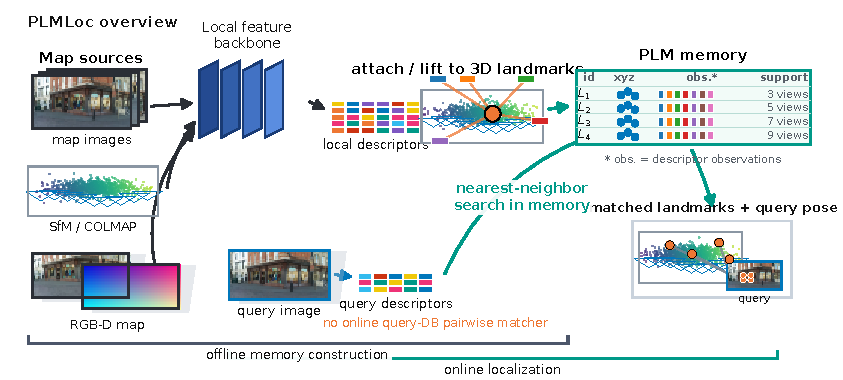
\includegraphics[width=0.98\textwidth]{figures/fig1_plm_pipeline_cvpr.pdf}
    \caption{Overview of \method. Offline, repeated local feature observations from an SfM/COLMAP map or an RGB-D map are attached or lifted to persistent 3D landmarks, then adaptive cover selects a variable descriptor subset per landmark. Online, retrieval selects a candidate map region, and query descriptors search the selected landmark observation memory to produce scored 2D--3D hypotheses for PnP-RANSAC.}
    \label{fig:plmloc-overview}
\end{figure*}

\section{Introduction}

Visual localization estimates the 6-DoF pose of a query image with respect to a mapped scene, typically by establishing 2D--3D correspondences between query keypoints and map landmarks and solving with robust PnP. Correspondence quality governs pose accuracy. Hierarchical localization retrieves database images, matches the query to retrieved views with learned pairwise matchers such as SuperGlue~\cite{sarlin2020superglue} or LightGlue~\cite{lindenberger2023lightglue}, and lifts the matches to 3D~\cite{sarlin2019hloc}; this is accurate but repeats online query--database matching at every query. Direct 2D--3D localization instead matches query features to descriptors associated with 3D points~\cite{sattler2011fast,sattler2012active}, avoiding the online matcher. Its limitation is that a single point descriptor compresses many observations: the same landmark is seen under different viewpoints, illumination, and sensor noise, and collapsing these observations discards appearance variation, while revisiting source images returns to pairwise matching. Direct localization therefore could benefit from a landmark-level representation that keeps descriptor diversity inside the map.

Scene-coordinate regression and pose-regression methods learn mappings from images to scene geometry or camera pose~\cite{brachmann2021dsacstar,brachmann2023ace}, but require scene-specific training or adaptation and often separate the learned model from an explicit reusable map. Rendering-based localization can exploit dense or learned scene representations~\cite{polizzi2025favor}, but typically introduces per-scene optimization or rendering machinery. RGB-D and SfM-free relocalization methods reduce the dependence on sparse reconstruction~\cite{glocker2013relocalization,dong2023lazyloc}, but may require depth or retain online pairwise matching. In contrast, repeated local-feature observations inside an explicit landmark representation remain comparatively underexplored: existing pipelines either revisit this evidence through source images at query time, compress it into compact point descriptors, or absorb it into scene-specific models.

\method{} addresses this by changing the landmark representation while keeping the standard sparse 2D--3D/PnP localization geometry. Each 3D landmark stores a bounded set of local descriptor observations, selected offline by adaptive coverage or fixed-budget selection. At query time, image retrieval only activates a relevant memory region; query descriptors are matched directly to selected landmark observations by mutual nearest-neighbor search, and accepted matches form 2D--3D hypotheses for a standard PnP-RANSAC backend. Thus, \method{} avoids online learned query--database matching while preserving explicit geometric verification.

The memory construction is map-source agnostic. For SfM/COLMAP maps, \method{} attaches local descriptors to existing 2D observations and 3D point identifiers. For posed RGB-D map frames, it backprojects local keypoints through depth and merges them into persistent world-space landmarks. This makes the representation applicable both to standard SfM-based localization pipelines and to robotic settings where posed RGB-D frames are available from SLAM or odometry.

Overall, our contributions are as follows:
\begin{itemize}[leftmargin=*,nosep]
\item We introduce adaptive-cover descriptor selection, a reliability-weighted submodular coverage rule with adaptive stopping that assigns each landmark a variable budget $K_p\in[K_{\min},K_{\max}]$ and retains only the observations needed to span its descriptor modes;

\item We show that adaptive cover matches all-observations accuracy while activating 0.40$\times$ the observations and about 0.56$\times$ the query time on Cambridge Landmarks, and uses about 2$\times$ fewer candidate observations than a fixed Farthest-16 budget;

\item We introduce \method{}, a training-free visual localization pipeline that matches RGB queries directly to persistent 3D landmark memory, avoiding online learned query--database pairwise matching;

\item We show that the same memory representation can be built from SfM/COLMAP observations or posed RGB-D frames; the standard RGB-only query path applies to both, with an optional RGB-D verification variant reported separately;

\item We report competitive results across indoor, outdoor, and large-scale localization benchmarks, with Cambridge and 7-Scenes performance on par with the best feature-matching baselines and large-scale gains over local-descriptor-only baselines.

\end{itemize}


\Cref{fig:plmloc-overview} gives the system overview, and \cref{alg:plmloc-query} summarizes query-time localization.

\begin{algorithm}[t]
\caption{\method{} Query-Time Localization}
\label{alg:plmloc-query}
\small
\begin{algorithmic}[1]
\Require Query image $I_q$, intrinsics $\mathbf{K}_q$, landmark memory $\mathcal{M}$, retrieval list $\mathcal{R}_q$, descriptor extractor $\phi$
\Ensure Camera pose $\hat{\mathbf{T}}_{wc}$
\State Extract query keypoints, scores, and $\ell_2$-normalized descriptors
       $Q=\{(\mathbf{u}_i,\alpha_i,\mathbf{q}_i)\}_{i=1}^{N_q}$ with $\phi$
\State Keep the top $K_r$ retrieved map frames
       $\mathcal{R}_q=(I_1,\ldots,I_{K_r})$
\State Activate candidate landmark ids observed in the retrieved frames:
       $\mathcal{P}_q \leftarrow \{p \mid \exists I_r\in\mathcal{R}_q,\ p\in\mathrm{obs}(I_r)\}$
\State For each $p\in\mathcal{P}_q$, expose selected memory observations using either a fixed $K_o$ or adaptive $K_p$
       $\mathcal{D}^{\star}_p\subseteq\mathcal{D}_p$
\State Build the active item bank
       $\mathcal{B}_q=\{(\mathbf{d}_{pm},\mathbf{x}_p,p)\mid p\in\mathcal{P}_q,\ \mathbf{d}_{pm}\in\mathcal{D}^{\star}_p\}$
\State $\mathcal{C}\leftarrow\emptyset$
\ForAll{$(\mathbf{u}_i,\alpha_i,\mathbf{q}_i)\in Q$}
    \State $(\mathbf{d}_{pm},\mathbf{x}_p,p) \leftarrow$ nearest item in $\mathcal{B}_q$ by cosine similarity
    \State $\mathbf{q}_{r} \leftarrow$ nearest query descriptor in $Q$ to $\mathbf{d}_{pm}$
    \If{$r=i$} \Comment{mutual nearest neighbors}
        \State $\mathcal{C}\leftarrow\mathcal{C}\cup\{(\mathbf{u}_i,\mathbf{x}_p,p)\}$
    \EndIf
\EndFor
\State Collapse repeated observations of the same $(i,p)$ pair, keeping the strongest score
\State Estimate $\hat{\mathbf{T}}_{wc}$ from $\mathcal{C}$ using two-stage PnP-RANSAC
\State \Return $\hat{\mathbf{T}}_{wc}$
\end{algorithmic}
\end{algorithm}

\section{Related Work}

\method{} follows the standard structure-based formulation of sparse 2D--3D correspondences to explicit 3D landmarks followed by PnP. The method focuses on how repeated descriptor observations are selected, stored, and searched as an explicit localization memory.

Classical direct 2D--3D localization matches query features to descriptors associated with 3D points. SIFT-based localization and direct matching methods~\cite{lowe2004sift,sattler2011fast} make this search efficient with visual vocabularies and prioritized correspondence search. Active Search~\cite{sattler2012active} further improves correspondence recovery using co-visibility and 2D-to-3D/3D-to-2D search. These methods establish the direct localization setting used by \method{}, but the landmark appearance is represented compactly at the point level. \method{} keeps the same explicit geometry, while retaining a bounded set of descriptor-diverse observations per landmark.

Hierarchical localization preserves source-image evidence differently. It retrieves database images, matches each retrieved view to the query with local matchers such as SuperGlue, LightGlue, or LoFTR~\cite{sarlin2020superglue,lindenberger2023lightglue,sun2021loftr}, and lifts the resulting matches to 3D~\cite{sarlin2019hloc,arandjelovic2016netvlad,sattler2018benchmarking,vislocbenchmark}. This gives strong correspondences, but the source evidence is revisited through online query--database matching. \method{} uses retrieval only to activate candidate landmarks, then matches query descriptors directly to stored landmark observations.

Several recent methods also reconsider how map evidence is used. FUSELOC~\cite{nguyen2024fuseloc} improves direct 2D--3D matching with a compact codebook that combines global and local cues. PRAM~\cite{xue2024pram} performs landmark-level recognition and verification. PixLoc~\cite{sarlin2021pixloc} refines camera pose by dense feature alignment to a 3D model rather than by sparse descriptor matching. FaVoR~\cite{polizzi2025favor} stores per-landmark descriptor evidence and synthesizes descriptors through per-scene voxel-rendering optimization. \method{} remains a sparse correspondence pipeline and stores observed descriptors directly, without per-scene training or rendering optimization.

RGB-D and SfM-free relocalization methods change how the map is obtained. Glocker et al.~\cite{glocker2013relocalization} build a relocalization database from RGB-D frames and localize RGB-D queries with hand-crafted descriptors. LazyLoc~\cite{dong2023lazyloc} and MAR-LOC~\cite{gassol2024marloc} reduce the need for SfM through sequence-level geometry, but still rely on online pairwise matching. ImLoc~\cite{jiang2026imloc} augments an image-based map with estimated depth. \method{} uses RGB-D as one possible source for building the same landmark observation memory. SfM/COLMAP provides 3D points through reconstruction, while posed RGB-D frames provide them by depth backprojection.

Scene-coordinate and pose-regression methods~\cite{shotton2013scene,brachmann2017dsac,brachmann2023ace,kendall2015posenet} encode scene geometry or camera pose in learned models and typically require scene-specific training or adaptation. \method{} keeps an explicit 3D map and uses standard geometric verification.


\section{Method}
\subsection{Landmark Observation Memory}
\method{} operates in the descriptor space of a frozen extractor $\phi$ (SuperPoint, ALIKED). A query image yields $Q=\{(\mathbf{u}_i,\alpha_i,\mathbf{q}_i)\}_{i=1}^{N_q}$ with keypoint $\mathbf{u}_i$, detector score $\alpha_i$, and descriptor $\mathbf{q}_i\in\mathbb{R}^{D}$. All descriptors are $\ell_2$ normalized before storage and matching; map and query descriptors are always compared within the same family and dimension $D$, so the similarity is the inner product (cosine). A landmark is a persistent 3D point and its descriptor observations,
\begin{equation}
\begin{aligned}
L_p &= (p,\mathbf{x}_p,\mathcal{O}_p,\mathcal{S}_p),\\
\mathcal{O}_p &= \{o_{pm}\}_{m=1}^{n_p}.
\end{aligned}
\label{eq:landmark-memory}
\end{equation}
Each observation is $o_{pm}=(\mathbf{d}_{pm},f_{pm},\mathbf{v}_{pm},\alpha_{pm})$ where $\mathbf{x}_p\in\mathbb{R}^3$ is the world coordinate, $\mathbf{d}_{pm}$ the normalized descriptor, $f_{pm}$ the source frame, and $\mathbf{v}_{pm}$ the source keypoint. $\mathcal{S}_p$ holds per-landmark statistics (observation count, source-frame count, descriptor variance, reprojection error, view diversity) used only for construction-time filtering. Memory is stored as contiguous per-landmark observation slices indexed by point id, with a per-image index so retrieval can activate landmarks by source image without scanning the full memory.

\subsection{Memory Construction}
Given a COLMAP reconstruction, \method{} attaches $\phi$ descriptors to existing observations. Points with track length below a minimum and/or reconstruction error above a threshold are discarded. For each map image, descriptors are attached in a \emph{feature-index} way, when the local-feature file matches the COLMAP feature order and the image-space discrepancy is within the attachment radius. When several detected features attach to one 3D point in an image, one is kept (lowest attachment distance, then highest detector score). Each accepted attachment adds one observation to landmark $p=p_\ell$ at $\mathbf{x}_p$.

\textbf{RGB-D.} Given posed RGB-D frames with intrinsics $\mathbf{K}$ and pose $\mathbf{T}_{wc}=(\mathbf{R}_{wc},\mathbf{t}_{wc})$, each keypoint with valid depth $z$ is lifted to world coordinates,
\begin{equation}
    \mathbf{x}_w=\mathbf{R}_{wc}\,z\mathbf{K}^{-1}[u,v,1]^\top+\mathbf{t}_{wc}.
    \label{eq:rgbd-backproject}
\end{equation}
 Lifted points are merged into landmarks by a metric radius $r_m$ using a voxel grid over centroids. Each point reuses the nearest centroid within $r_m$ (centroid updated by running mean) or creates a new landmark. As in the SfM path, only the strongest observation per landmark per source frame is kept. The output has the same array format as the SfM memory, so the query-time localizer is identical. Depth is used only to build the map; queries use RGB descriptors and PnP.

\subsection{Observation Selection}
Each landmark exposes a bounded subset $\mathcal{D}^{\star}_p$ of its observations. Fixed-budget selection uses a global budget $K_o$: if $n_p\le K_o$, all observations are exposed; otherwise a selection rule keeps $K_o$ observations. We use fixed Farthest, First, Random, and All-observations variants as controls, and distinguish them from the adaptive rule below. Farthest starts from the descriptor closest to the normalized landmark mean and greedily adds the observation farthest from the selected set under cosine distance. The point-mean baseline differs from $K_o=1$ because it collapses all observations to a single normalized mean descriptor.

\textbf{Adaptive cover.}
A fixed observation budget assigns the same memory size to every landmark, although landmarks differ substantially in appearance complexity. We therefore also evaluate an adaptive-cover selection rule that chooses a landmark-specific budget $K_p$. For landmark $p$, each observation receives a reliability weight from its detector score, attachment distance, and reprojection error:
\[
\begin{aligned}
\tilde{w}_{pm}
&=
\bar{\alpha}_{pm}
\exp\!\left(-\frac{\delta_{pm}^{2}}{2\sigma_a^2}\right)
\exp\!\left(-\frac{\epsilon_{pm}^{2}}{2\sigma_r^2}\right),\\
w_{pm}
&=
\frac{\tilde{w}_{pm}}{\sum_j\tilde{w}_{pj}} .
\end{aligned}
\]
Here $\bar{\alpha}_{pm}$ is normalized within the landmark, $\delta_{pm}$ is the 2D attachment distance to the COLMAP observation, and $\epsilon_{pm}$ is the reprojection error. Missing scores fall back to uniform weights, and unavailable error terms are omitted from the penalty.

Adaptive cover then greedily maximizes weighted descriptor coverage. With normalized descriptors, we use
\[
s_{mn}=\frac{1+\mathbf{d}_{pm}^{\top}\mathbf{d}_{pn}}{2},
\qquad
F(A)=\sum_m w_{pm}\max_{a\in A}s_{ma}.
\]
The first selected observation is the weighted medoid,
\[
a_1=\operatorname*{arg\,max}_n \sum_m w_{pm}s_{mn},
\]
and each subsequent observation maximizes the marginal coverage gain
\[
\Delta(n\mid A)=
\sum_m w_{pm}\max\!\left(0,s_{mn}-\max_{a\in A}s_{ma}\right).
\]
Selection stops once the gain falls below $\tau$, after at least $K_{\min}$ observations, or when $K_{\max}$ is reached. In our experiments we use $K_{\min}=1$, $K_{\max}=32$, $\tau=0.005$, $\sigma_a=2.0$, and $\sigma_r=4.0$. Thus stable landmarks keep compact memories, while landmarks with multiple appearance modes retain more observations. Since $F$ is a monotone submodular facility-location coverage function and $\Delta$ is its marginal gain, greedy selection of a fixed budget $K_{\max}$ attains the standard $(1-1/e)$ guarantee relative to the optimal $K_{\max}$-cardinality coverage; the threshold $\tau$ then stops early, trading a small amount of coverage for reduced memory.

\subsection{Query-Time Localization}
Retrieval returns an ordered list $\mathcal{R}_q$ of $K_r$ database images. \method{} uses it only to restrict the candidate region where the active landmarks $\mathcal{P}_q$ are the unique point ids observed in any retrieved image, and the active bank is
\begin{equation}
    \mathcal{B}_q=\{(\mathbf{d}_{pm},\mathbf{x}_p,p)\mid p\in\mathcal{P}_q,\ \mathbf{d}_{pm}\in\mathcal{D}^{\star}_p\}.
\end{equation}

Correspondences use mutual nearest-neighbor matching between query descriptors and $\mathcal{B}_q$: a match $(\mathbf{q}_i,\mathbf{b}_m)$ is accepted iff each is the other's nearest neighbor,
\begin{equation}
    i^{\star}(m^{\star}(i))=i,
    \qquad
    m^{\star}(i)=\operatorname*{arg\,max}_{m}\mathbf{q}_i^{\top}\mathbf{b}_m,
    \label{eq:mnn}
\end{equation}
Each accepted item lifts to a hypothesis $(\mathbf{u}_i,\mathbf{x}_{p(m^{\star}(i))})$; duplicate $(\text{query},\text{landmark})$ pairs are collapsed by descriptor score. We do not impose a global one-to-one landmark assignment; repeated-structure hypotheses are left for the geometric backend to reject. Finally, pose is estimated by two-stage PnP-RANSAC. When multiple retrieval clusters are evaluated, the pose with the most inliers is selected.

\section{Experiments}

We evaluate whether descriptor-diverse landmark memory is a useful correspondence target for visual localization. The experiments are organized around four points. First, we compare \method{} with feature-matching, render-based, scene-coordinate, and pose-regression baselines on standard indoor and outdoor benchmarks. Second, we isolate the effect of replacing online query--database matching with direct query-to-memory matching. Third, we test whether the same memory format can be populated from either SfM/COLMAP observations or posed RGB-D frames. Finally, we study the effect of observation budget, selection strategy, retrieval budget, runtime, and memory footprint.

\begin{table*}[!t]
    \centering
    \caption{Localization comparison on Cambridge Landmarks. We report median translation and rotation errors in cm/$^\circ$. FM denotes feature matching, SFRM render-based / feature-rendering methods, E2E end-to-end localization, and SCR scene-coordinate regression. FaVoR requires per-scene voxel optimization. DSAC$^\ast$ variants follow the taxonomy of the cited sources. Rows marked $^\ast$ are reproduced from ImLoc~\cite{jiang2026imloc}. Baseline values are quoted at the precision reported in their sources, whereas \method{} averages are computed from per-scene medians.}
    \label{tab:cambridge-results}
    \setlength{\tabcolsep}{2.4pt}
    \begin{adjustbox}{max width=\textwidth}
    \begin{tabular}{@{}llcccccc@{}}
        \toprule
        Family & Method & Court & King's & Hospital & Shop & St. Mary's & Avg. $\downarrow$ \\
        \midrule
        \multirow{10}{*}{FM}
        & \textbf{Ours (SP+MNN)} & \textbf{14.52/0.09} & \textbf{10.15/0.18} & \textbf{12.43/0.28} & \underline{4.08/0.19} & \textbf{6.54/0.21} & \textbf{9.55/0.19} \\
        & \textbf{Ours (ALIKED+MNN)} & \underline{14.66/0.09} & \underline{10.54/0.19} & \underline{12.55/0.26} & 4.36/0.19 & \underline{6.63/0.22} & \underline{9.75/0.19} \\
        & FUSELOC (light, D2+MixVPR, $\lambda{=}0.5$)~\cite{nguyen2024fuseloc} & 16/0.1 & 11/0.2 & 14/0.3 & \textbf{4/0.2} & \textbf{6/0.2} & 10/0.2 \\
        & ImLoc~\cite{jiang2026imloc}$^\ast$ & 16/0.1 & 11/0.2 & 14/0.3 & \textbf{4/0.2} & 7/0.2 & 10/0.2 \\
        & HLoc (SP+SG)~\cite{sarlin2019hloc,sarlin2020superglue}$^\ast$ & 16/0.1 & 12/0.2 & 15/0.3 & \textbf{4/0.2} & 7/0.2 & 11/0.2 \\
        & HLoc (SP+LG)~\cite{sarlin2019hloc,lindenberger2023lightglue}$^\ast$ & 18/0.1 & 12/0.2 & 15/0.3 & \textbf{4/0.2} & 7/0.2 & 11/0.2 \\
        & HLoc (ALIKED+LG)~\cite{lindenberger2023lightglue,zhao2023aliked}$^\ast$ & 19/0.1 & 13/0.2 & 16/0.3 & \textbf{4/0.2} & 7/0.2 & 12/0.2 \\
        & HLoc (RoMa)~\cite{edstedt2024roma}$^\ast$ & 17/0.1 & 15/0.2 & 17/0.3 & 7/0.3 & 8/0.2 & 13/0.2 \\
        & AS (SIFT)~\cite{sattler2012active}$^\ast$ & 24/0.1 & 13/0.2 & 20/0.4 & \textbf{4/0.2} & 8/0.3 & 14/0.2 \\
        & PixLoc~\cite{sarlin2021pixloc}$^\ast$ & 30/0.1 & 14/0.2 & 16/0.3 & 5/0.2 & 10/0.3 & 15/0.2 \\
        \midrule
        \multirow{2}{*}{SFRM}
        & FaVoR (ALIKED-l)~\cite{polizzi2025favor} & 27/0.1 & 15/0.2 & 19/0.4 & 5/0.3 & 10/0.3 & 15/0.3 \\
        & FaVoR (SuperPoint)~\cite{polizzi2025favor} & 29/0.2 & 18/0.3 & 27/0.5 & 5/0.3 & 11/0.4 & 18/0.3 \\
        \midrule
        \multirow{3}{*}{E2E}
        & SC-wLS~\cite{wu2022scwls} & 29/0.2 & \textbf{8/0.2} & \textbf{11/0.4} & \underline{4/0.3} & 9/0.3 & 12/0.3 \\
        & NG-DSAC~\cite{brachmann2019ngdsac} & 35/0.2 & 12/0.2 & 21/0.5 & 5/0.3 & 10/0.3 & 17/0.3 \\
        & DSAC$^\ast$~\cite{brachmann2021dsacstar} & 34/0.2 & 18/0.3 & 21/0.4 & 5/0.3 & 15/0.6 & 19/0.4 \\
        \midrule
        \multirow{4}{*}{SCR}
        & GLACE~\cite{wang2024glace}$^\ast$ & 19/0.1 & 19/0.3 & 17/0.4 & \textbf{4/0.2} & 9/0.3 & 14/0.3 \\
        & Poker (ACE~\cite{brachmann2023ace} $\times 4$)$^\ast$ & 28/0.1 & 18/0.3 & 25/0.5 & 5/0.3 & 9/0.3 & 17/0.3 \\
        & DSAC$^\ast$ (Full)~\cite{brachmann2021dsacstar}$^\ast$ & 49/0.3 & 15/0.3 & 21/0.4 & 5/0.3 & 13/0.4 & 21/0.3 \\
        & ACE~\cite{brachmann2023ace}$^\ast$ & 43/0.2 & 28/0.4 & 31/0.6 & 5/0.3 & 18/0.6 & 25/0.4 \\
        \bottomrule
    \end{tabular}
    \end{adjustbox}
\end{table*}
\subsection{Datasets and Metrics}

Cambridge Landmarks evaluates outdoor localization from registered image sequences~\cite{kendall2015posenet}. We report median translation and rotation errors in cm/$^\circ$ on all five scenes.

7-Scenes evaluates indoor relocalization from RGB-D sequences~\cite{microsoft7scenes}. The main \method{} rows use SfM-built SuperPoint maps and RGB-only PnP localization. For the map-source comparison in \cref{tab:rgbd-vs-sfm}, we additionally report RGB-D-built landmark memory; the query-depth column specifies whether depth is used during pose verification.

We also report Visual Localization benchmark results on Aachen Day/Night v1.1, RobotCar Seasons v2, and Extended CMU Seasons in \cref{tab:vloc-large-scale-reference}. Following the benchmark convention, we report the percentage of query images localized under the standard pose-error thresholds.


\subsection{Baselines and Experimental Protocol}

The primary controlled comparison is against lifted image-pair localization pipelines that use the same retrieval, map, and PnP backend whenever possible, but obtain correspondences through online pairwise matching with SuperGlue or LightGlue. This separates the query-time correspondence source from the rest of the localization pipeline.

We also compare with published feature-matching, render-based, scene-coordinate-regression, and pose-regression methods. These methods may use different maps, features, training data, or scene representations, so we treat them as reference results under the same benchmark protocols rather than as fully controlled ablations. For FUSELOC, we report the best published flavor without rerunning its codebook training.

All headline \method{} rows use frozen local features, Top-10 MixVPR retrieval~\cite{alibey2023mixvpr,berton2025megaloc}, and adaptive-cover landmark memory ($K_{\min}=1$, $K_{\max}=32$, $\tau=0.005$), so their accuracies and map footprints come from the same selected memory. SuperPoint descriptors use 4096 keypoints per image. Fixed-budget Farthest, First, Random, and All-observations variants appear only as controls in \cref{tab:ablation-budget}. Query descriptors are matched to active landmark observations by mutual nearest-neighbor search, and poses are estimated with a two-stage PnP-RANSAC backend. Landmark memory is built from the map split only.

\subsection{Cambridge Landmarks}

\Cref{tab:cambridge-results} reports median translation and rotation errors on Cambridge Landmarks. \method{} with ALIKED+MNN is competitive with the best feature-matching baselines in this table. Because the leading methods are separated by very small margins and are reported from different sources, we interpret Cambridge as a parity result rather than a decisive ranking. It also compares favorably with the FaVoR variants on this benchmark, while avoiding their per-scene voxel optimization.

\Cref{tab:cambridge-matcher-split} focuses on the correspondence source and stored map representation. \method{} replaces online query--database matching with direct matching to landmark observation memory. The ALIKED+MNN and SP+MNN rows show that this direct memory search remains competitive with strong online matching pipelines, while removing the learned pairwise matcher from the query-time loop.


\Cref{tab:cambridge-matcher-split} compares \method{} memory search with the Cambridge matcher/map-size comparison reported by ImLoc~\cite{jiang2026imloc}.

\begin{table*}[!t]
    \centering
    \caption{Cambridge Landmarks comparison by map construction, query-time correspondence source, and stored map size. We report median translation and rotation errors in cm/$^\circ$. Published HLoc, LoFTR, RoMa, and ImLoc map-size values are reproduced as stored reference-map footprints reported by ImLoc~\cite{jiang2026imloc}; they are not top-$k$ query-activated subsets. For \method{}, map size is the approximate five-scene average adaptive-cover float16 landmark-memory array footprint; the per-query activated subset is reported separately in \cref{tab:runtime}.}
    \label{tab:cambridge-matcher-split}
    \setlength{\tabcolsep}{2.4pt}
    \begin{adjustbox}{max width=\textwidth}
    \begin{tabular}{@{}llllcccccc@{}}
        \toprule
        Method & Mapping matcher & Query matcher & Stored map size & Court & King's & Hospital & Shop & St. Mary's & Avg. $\downarrow$ \\
        \midrule
        \textbf{Ours (SP+MNN)} & SP+SG & Memory MNN & $\sim$287MB & \textbf{14.52/0.09} & \textbf{10.15/0.18} & \textbf{12.43/0.28} & \underline{4.08/0.19} & \textbf{6.54/0.21} & \textbf{9.55/0.19} \\
        \textbf{Ours (ALIKED+MNN)} & ALIKED+LG & Memory MNN & $\sim$220MB & \underline{14.66/0.09} & \underline{10.54/0.19} & \underline{12.55/0.26} & 4.36/0.19 & \underline{6.63/0.22} & \underline{9.75/0.19} \\
        \midrule
        HLoc (SP+LG)~\cite{sarlin2019hloc,lindenberger2023lightglue} & SP+LG & SP+LG & $\sim$800MB & 18/0.1 & 12/0.2 & 15/0.3 & \textbf{4/0.2} & \underline{7/0.2} & 11/0.2 \\
        LoFTR~\cite{sun2021loftr} & LoFTR & LoFTR & $\sim$360MB & 16/0.1 & 13/0.2 & 16/0.3 & \textbf{4/0.2} & 8/0.2 & 12/0.2 \\
        RoMa~\cite{edstedt2024roma} & RoMa & RoMa & $\sim$300MB & 17/0.1 & 15/0.2 & 17/0.3 & 7/0.3 & 8/0.2 & 13/0.2 \\
        \midrule
        ImLoc~\cite{jiang2026imloc} & RoMa & SP+LG & $\sim$90MB & 17/0.1 & 11/0.2 & 14/0.3 & \textbf{4/0.2} & \underline{7/0.2} & 11/0.2 \\
        ImLoc~\cite{jiang2026imloc} & RoMa & LoFTR & $\sim$90MB & 17/0.1 & 11/0.2 & 13/0.3 & \textbf{4/0.2} & 7/0.2 & 10/0.2 \\
        ImLoc~\cite{jiang2026imloc} & RoMa & RoMa & $\sim$90MB & \underline{16/0.1} & 11/0.2 & 14/0.3 & \textbf{4/0.2} & \underline{7/0.2} & \underline{10/0.2} \\
        \bottomrule
    \end{tabular}
    \end{adjustbox}
\end{table*}

\subsection{7-Scenes}

\Cref{tab:seven-scenes-results} reports 7-Scenes localization with a per-scene training column. Among methods without per-scene training, \method{} is on par with the best feature-matching baselines; the average translation differences among \method{}, DVLAD+R2D2, and HLoc are small. Render-based and scene-coordinate-regression methods obtain lower indoor errors, but require per-scene optimization or training. The main conclusion is that \method{} remains competitive while avoiding online pairwise matching.



\begin{table*}[!t]
    \centering
    \caption{Localization comparison on 7-Scenes with per-scene training cost. We report median translation and rotation errors in cm/$^\circ$ and average over all seven scenes. ``Per-scene training'' indicates offline optimization required per scene beyond providing database poses. FaVoR and DSAC$^\ast$ require per-scene optimization; \method{}, HLoc, AS, and DVLAD+R2D2 do not.}
    \label{tab:seven-scenes-results}
    \setlength{\tabcolsep}{2.4pt}
    \begin{adjustbox}{max width=\textwidth}
    \begin{tabular}{@{}llccccccccc@{}}
        \toprule
        Family & Method & Per-scene training & Chess & Fire & Heads & Office & Pumpkin & RedKitchen & Stairs & Avg. $\downarrow$ \\
        \midrule
        SFRM & FaVoR (ALIKED-l)~\cite{polizzi2025favor} & voxel opt. & \textbf{1/0.2} & \textbf{1/0.3} & 1/0.4 & \textbf{2/0.4} & \textbf{1/0.3} & \textbf{1/0.2} & \textbf{3/0.8} & \textbf{1.4/0.4} \\
        SFRM & FaVoR (SuperPoint)~\cite{polizzi2025favor} & voxel opt. & \textbf{1/0.2} & \underline{1/0.4} & \underline{1/0.3} & \textbf{2/0.4} & \textbf{1/0.3} & \textbf{1/0.2} & \underline{4/1.0} & \underline{1.6/0.4} \\
        \midrule
        SCR & DSAC$^\ast$~\cite{brachmann2021dsacstar} & hours & \underline{1.9/1.11} & 1.9/1.24 & 1.1/1.82 & \underline{2.6/1.18} & 4.2/1.41 & \underline{3.0/1.70} & 4.1/1.42 & 2.7/1.41 \\
        \midrule
        FM & \textbf{Ours (ALIKED+MNN)} & \textbf{none} & 2.35/0.77 & 2.12/0.89 & 1.19/0.79 & 2.93/0.82 & \underline{3.97/1.10} & 3.95/1.26 & 5.73/1.50 & 3.18/1.02 \\
        FM & DVLAD+R2D2~\cite{revaud2019r2d2} & none & 2.56/0.88 & 2.21/0.86 & \textbf{0.98/0.75} & 3.48/1.00 & 4.79/1.28 & 4.21/1.44 & 4.60/1.27 & 3.26/1.07 \\
        FM & \textbf{Ours (SP+MNN)} & \textbf{none} & 2.52/0.83 & 2.06/0.83 & 1.13/0.78 & 3.11/0.89 & 4.72/1.30 & 4.41/1.35 & 5.29/1.39 & 3.32/1.05 \\
        FM & HLoc (SP+SG)~\cite{sarlin2019hloc,sarlin2020superglue} & none & 2.39/0.84 & 2.29/0.91 & 1.13/0.77 & 3.14/0.92 & 4.92/1.30 & 4.22/1.39 & 5.05/1.41 & 3.31/1.08 \\
        FM & AS (SIFT)~\cite{sattler2012active} & none & 3/0.87 & 2/1.01 & 1/0.82 & 4/1.15 & 7/1.69 & 5/1.72 & 4/1.01 & 3.71/1.18 \\
        \bottomrule
    \end{tabular}
    \end{adjustbox}
\end{table*}

\subsection{SfM and RGB-D Map Construction}

\Cref{tab:rgbd-vs-sfm} compares two ways of building landmark memory on 7-Scenes. The SfM row attaches local descriptors to SuperPoint+SuperGlue SfM points and localizes RGB queries with PnP. The RGB-D row builds landmarks directly from posed RGB-D frames and uses the RGB-D 3D--3D verification backend. This experiment tests the map-construction interface rather than claiming identical query modalities. The average results show that RGB-D frames can populate a comparable landmark memory with fewer landmarks, while the table explicitly marks the use of query depth in the RGB-D verification setting.


\begin{table*}[!t]
    \centering
    \caption{Average map-source comparison on 7-Scenes: SfM-built vs. RGB-D-built landmark memory. We report median translation (cm), median rotation ($^\circ$), and whether depth is used during pose verification.}
    \label{tab:rgbd-vs-sfm}
    \setlength{\tabcolsep}{4pt}
    \begin{adjustbox}{max width=\textwidth}
    \begin{tabular}{@{}llccccc@{}}
        \toprule
        Scene & Map source & Med. trans (cm) & Med. rot ($^\circ$) & \#landmarks & Map build time & Query depth \\
        \midrule
        7-Scenes Avg. & SfM (SP+SG) & \textbf{3.28} & \textbf{1.04} & \underline{1{,}085{,}992} & -- & No \\
        7-Scenes Avg. & RGB-D (3D--3D) & \underline{3.30} & \underline{1.84} & \textbf{489{,}110} & -- & Yes \\
        \bottomrule
    \end{tabular}
    \end{adjustbox}
    \\[2pt]
    {Map build time is the \method{} landmark-memory construction step after the source SfM/RGB-D map is available; elapsed build time was not recorded for these runs.}
\end{table*}

\subsection{Runtime and Memory}

\Cref{tab:runtime} reports online correspondence search and pose-estimation cost, excluding query descriptor extraction. \method{} stores landmark-memory descriptors directly and avoids running a learned pairwise matcher for each retrieved image. On the reported OldHospital runs, the SP+MNN configuration has the lowest query time, while ALIKED+MNN remains faster than the listed HLoc pairwise baselines. The candidate counts are not directly comparable across methods because \method{} counts active memory observations, whereas HLoc counts lifted 2D--3D correspondences.


\begin{table*}[!t]
    \centering
    \caption{Runtime and memory diagnostics on matched hardware. Runtime excludes query descriptor extraction and measures online correspondence search plus pose estimation.}
    \label{tab:runtime}
    \setlength{\tabcolsep}{5pt}
    \begin{adjustbox}{max width=\textwidth}
    \begin{tabular}{@{}lccccc@{}}
        \toprule
        Method & Stored map (MB) & Cand. obs/query & Query time (s) & FPS & Peak RAM (MB) \\
        \midrule
        Ours (ALIKED+MNN) & \textbf{293} & 42{,}431 & \underline{0.25} & \underline{4.02} & 2{,}160 \\
        Ours (SP+MNN) & \underline{346} & 21{,}065 & \textbf{0.11} & \textbf{9.21} & 2{,}396 \\
        HLoc (SP+SG)~\cite{sarlin2019hloc,sarlin2020superglue} & 1{,}718 & \textbf{1{,}459} & 0.73 & 1.36 & \underline{2{,}072} \\
        HLoc (SP+LG)~\cite{sarlin2019hloc,lindenberger2023lightglue} & 1{,}718 & \underline{1{,}463} & 0.32 & 3.15 & \textbf{2{,}056} \\
        \bottomrule
    \end{tabular}
    \end{adjustbox}
    \\[2pt]
    {Results are OldHospital runs. For \method{}, stored map size is the approximate OldHospital adaptive-cover float16 landmark-memory footprint, whereas \cref{tab:cambridge-matcher-split} reports the five-scene average; candidates are active memory observations/query. For HLoc, map size is the stored SuperPoint feature file plus SfM model, and candidates are lifted 2D--3D correspondences/query.}
\end{table*}

\subsection{Observation Budget and Selection}

The ablation in \cref{tab:ablation-budget} reports a Cambridge-wide observation-budget study for Ours (SP+MNN), using Top-5 MegaLoc retrieval and macro-averaging over the five Cambridge scenes. The fixed Farthest-8 descriptor-diverse memory gives the best macro median error and strict recall among the completed variants, while activating roughly half as many candidate observations as all-observations memory. Increasing the fixed budget beyond eight observations gives no accuracy benefit on average. Adaptive cover variants remain useful compact-memory controls, especially adaptive cover v2, which substantially reduces candidate observations, but they do not improve the five-scene median error in this run.

The first-$k$ and random rows provide selection-rule controls at $K_o{=}16$. They remain close to the farthest rows, indicating that large enough fixed budgets can mask the selection rule, but Farthest-8 is the best accuracy--candidate tradeoff in the completed grid.

\begin{table*}[!t]
    \centering
    \caption{Absolute observation-budget and selection ablation for Ours (SP+MNN) on Cambridge Landmarks with Top-5 MegaLoc retrieval. Values are macro-averages over the five scenes. $K_o$ is the maximum number of exposed observations per landmark; adaptive variants use a variable $K_p$. Strict recall is measured at 25\,cm and 2$^\circ$. Candidate observations are averaged from per-scene run summaries. Query times are adjusted from mounted-disk runs by a $3.5\times$ local-disk speed factor. Lower error, fewer candidates, and lower time are better.}
    \label{tab:ablation-budget}
    \setlength{\tabcolsep}{3.5pt}
    \begin{adjustbox}{max width=\textwidth}
    \begin{tabular}{@{}llcccccc@{}}
        \toprule
        Selection & $K_o$ & Avg. med. trans (cm) & Avg. med. rot ($^\circ$) & Strict (\%) & Avg. $K_p$ & Cand. obs/query & Query time (s) \\
        \midrule
        Farthest-point        & 8     & \textbf{9.55} & 0.19 & \textbf{81.9} & 4.89 & 27{,}225 & \underline{0.36} \\
        First-$k$             & 16    & \underline{9.61} & 0.19 & 81.0 & 6.02 & 39{,}337 & 0.37 \\
        Random                & 16    & 9.66 & 0.19 & 81.4 & 6.02 & 39{,}337 & 0.38 \\
        Farthest-point        & 32    & 9.70 & 0.19 & 81.1 & 6.51 & 47{,}529 & 0.43 \\
        Farthest-point        & 16    & 9.70 & 0.19 & 80.8 & 6.02 & 39{,}337 & 0.41 \\
        Point mean            & 1     & 9.72 & 0.19 & 81.3 & \textbf{1.00} & \textbf{4{,}275} & \textbf{0.19} \\
        Adaptive cover v2     & 1--12 & 9.76 & 0.19 & \underline{81.8} & \underline{2.14} & \underline{12{,}104} & 0.72 \\
        Farthest-point        & 12    & 9.81 & 0.19 & 81.6 & 5.63 & 34{,}548 & 0.39 \\
        Adaptive cover        & 1--32 & 9.84 & 0.19 & 81.3 & 3.79 & 21{,}204 & 0.67 \\
        All observations      & all   & 9.89 & 0.19 & 81.4 & 6.68 & 52{,}171 & 0.44 \\
        \bottomrule
    \end{tabular}
    \end{adjustbox}
    \\[2pt]
    {Query time excludes feature extraction and includes online correspondence search plus pose estimation. Candidate observations are active memory observations/query. Per-budget query times are averaged over a small number of runs and are dominated by system variance (Farthest-16 vs Farthest-32 is non-monotonic); candidate counts are the deterministic efficiency measure.}
\end{table*}

\subsection{Large-Scale Localization}

\Cref{tab:vloc-large-scale-reference} places \method{} on Aachen Day/Night v1.1, RobotCar Seasons v2, and Extended CMU Seasons. \method{} with ALIKED+MNN is competitive with the HLoc reference on average, improves over the listed local-descriptor-only baselines by a substantial margin, and gives the best strict-threshold RobotCar result in the table. HLoc remains stronger on several Aachen thresholds, which is expected for a hierarchical pipeline with online learned pairwise matching. These results support the main claim that descriptor-diverse landmark memory can be a competitive query-time correspondence target without per-scene training or online query--database matching.

\begin{table*}[!t]
    \centering
    \caption{Visual Localization benchmark results on Aachen Day/Night v1.1, RobotCar Seasons v2, and Extended CMU Seasons. Values are the percentage of query images successfully localized under each threshold; best results are bold and second-best results are underlined. The average summarizes the reported dataset-threshold entries. The Ours (ALIKED+MNN) RobotCar result is all-query weighted, and Extended CMU results reported from urban, suburban, and park are macro-averages over the three subsets.}
    \label{tab:vloc-large-scale-reference}
    \setlength{\tabcolsep}{2.0pt}
    \begin{adjustbox}{max width=\textwidth}
    \begin{tabular}{@{}lcccccccccc@{}}
        \toprule
        & \multicolumn{3}{c}{Aachen Day/Night v1.1} & \multicolumn{3}{c}{RobotCar Seasons v2} & \multicolumn{3}{c}{Extended CMU Seasons} & \multirow{2}{*}{Avg. $\uparrow$} \\
        \cmidrule(lr){2-4}\cmidrule(lr){5-7}\cmidrule(lr){8-10}
        Method & 0.25m/2$^\circ$ & 0.5m/5$^\circ$ & 5m/10$^\circ$ & 0.25m/2$^\circ$ & 0.5m/5$^\circ$ & 5m/10$^\circ$ & 0.25m/2$^\circ$ & 0.5m/5$^\circ$ & 5m/10$^\circ$ & \\
        \midrule
        \textbf{Ours (ALIKED+MNN)} & \underline{82.8} & \underline{93.2} & \underline{99.4} & \textbf{56.5} & \textbf{91.3} & \textbf{99.4} & \textbf{92.0} & \textbf{95.4} & \textbf{98.8} & \textbf{89.9} \\
        HLoc (SP+SG)~\cite{sarlin2019hloc,sarlin2020superglue} & \textbf{83.4} & \textbf{93.4} & \textbf{99.7} & \underline{52.0} & \underline{87.2} & \underline{96.1} & \underline{90.7} & \underline{93.9} & \underline{96.0} & \underline{88.0} \\
        \textbf{Ours (SP+MNN)} & 77.0 & 89.6 & 97.1 & 46.6 & 77.0 & 95.7 & 86.4 & 89.4 & 95.2 & 83.8 \\
        PixLoc~\cite{sarlin2021pixloc} & 81.7 & 91.5 & 97.8 & 45.8 & 68.6 & 89.3 & 76.3 & 78.0 & 82.8 & 79.1 \\
        FUSELOC (light, D2+MixVPR)~\cite{nguyen2024fuseloc} & 72.4 & 81.4 & 89.0 & 37.4 & 64.7 & 76.6 & 83.0 & 88.1 & 93.9 & 76.3 \\
        D2-Net~\cite{dusmanu2019d2net} & 72.6 & 80.4 & 87.7 & 36.4 & 63.7 & 74.8 & 78.8 & 83.0 & 89.8 & 74.2 \\
        SuperPoint~\cite{detone2018superpoint} & 67.4 & 77.7 & 85.6 & 31.0 & 51.4 & 61.1 & 60.1 & 65.0 & 72.6 & 63.5 \\
        R2D2~\cite{revaud2019r2d2} & 68.9 & 76.7 & 85.7 & 32.4 & 51.8 & 59.4 & 55.9 & 60.1 & 68.6 & 62.2 \\
        CSL~\cite{svarm2017csl} & 48.0 & 72.6 & 87.1 & 35.1 & 57.3 & 71.1 & 54.5 & 57.8 & 62.8 & 60.7 \\
        SIFT~\cite{lowe2004sift} & 56.0 & 60.0 & 65.6 & 24.9 & 39.2 & 43.6 & 34.6 & 38.6 & 45.4 & 45.3 \\
        ESAC~\cite{brachmann2019esac} & 35.7 & 50.3 & 64.8 & -- & -- & -- & -- & -- & -- & -- \\
        AS~\cite{sattler2012active} & 76.7 & 84.1 & 91.6 & 34.0 & 60.3 & 75.7 & 63.0 & 69.9 & 78.5 & -- \\
        GLACE~\cite{wang2024glace} & 4.8 & 10.9 & 40.6 & -- & -- & -- & -- & -- & -- & -- \\
        \bottomrule
    \end{tabular}
    \end{adjustbox}
\end{table*}

\subsection{Retrieval Budget}

We study how many retrieved frames should activate the memory. On Cambridge ShopFacade, top-5 and top-10 retrieval give the same rounded median translation error of $4.04$\,cm, while top-50 increases the active memory to $99.0$k observations per query and slightly worsens the median error to $4.29$\,cm. A small retrieval budget is therefore sufficient for this scene, whereas larger budgets can add distractors and query cost.

\section{Discussion and Conclusion}

\method{} revisits direct 2D--3D localization through the map representation rather than through a new pose solver. Instead of compressing each 3D point to one descriptor or revisiting source images with an online query--database matcher, \method{} stores a compact selected set of landmark observations and searches this memory directly. Adaptive cover assigns the observation budget per landmark, matching all-observations accuracy on Cambridge while using substantially fewer active candidates and lower query time. Across indoor, outdoor, and large-scale benchmarks, the results indicate that descriptor-diverse landmark memory is a competitive correspondence target for RGB-only localization without per-scene training or an online learned pairwise matcher.

The representation is also independent of how landmarks are obtained. With SfM/COLMAP maps, \method{} attaches descriptors to existing 2D--3D observations and inherits the coverage and accuracy of the reconstruction. With posed RGB-D map frames, it backprojects local features into persistent landmarks, avoiding triangulation but depending on accurate map-frame poses, reliable depth, and an appropriate merge radius. The standard query path remains RGB-only and uses PnP. The reported RGB-D 3D--3D row uses query depth and should therefore be read as a separate verification setting, not as the default operating mode.

The main failure modes are retrieval misses, insufficient appearance coverage in the stored observations, and active-memory search cost. Severe day--night changes remain challenging because mutual nearest-neighbor descriptor search lacks the pair-specific context of learned online matchers. Adaptive cover also uses a global stopping threshold $\tau$, which may not be optimal for every scene or landmark. Future work should index or compress the active memory, improve robustness under large appearance change, and combine persistent landmark memory with stronger retrieval and prioritized correspondence search.

\bibliographystyle{unsrt}
\bibliography{references}

\end{document}
